%!TEX root = thesis.tex
%=============================================================================


\chapter{Concepts and Technologies}
\label{basics:start}
In this chapter, I will provide an overview of and describe concepts and technologies used within this work.
First, latency will be discussed, as it is important when designing the resulting framework.
Then the concepts of \gls{asr}, \gls{ssl} and beamforming are introduced.
They are later incorporated into the resulting framework, or are at least considered during its design.
Finally, \gls{ros} will be discussed, as it was chosen as middleware. 
The reasons for this will be discussed in chapter \ref{main:main}.


\section{Latency}
\label{basics:latency}
Regardless of the method used, when transmitting any kind of information, this transmission will not be instantaneous, but instead happen with a delay.
This delay is a universal effect and can be found in macro levels, light from distant galaxies reaching us after thousands of years, over a more intermediate level, sending a letter to a micro level, the sound of a spoken phrase to reach the ear of the recipient.
This delay is also known as \textit{latency}.

However, while the laws of physics cannot be altered, one might be able to reduce latency when in control of the environment.
To follow the previous example of sending a letter, one may opt for sending an intercontinental letter via plane instead of ship.

In this work, latency will be discussed in the context of transmitting audio signals.
As audio signals are not singular events, akin to e.g. a photon, but rather a continuous stream and most of the computations presented in this work are done by computers which can work faster then audio signals typically occur, their latency behaves differently in a number of ways. % todo formulierung
One such special behavior for example can be observed when recording audio from a microphone.
This is typically done in an iterative manner:
the software will require a predetermined number of audio frames, i.e. singular data points of an audio stream.
After these frames are acquired, they can be processed.
Then, it will typically wait for the next batch of available data.
Through this procedure, the amount of frames requested can have a impact on the overall latency measured.
Consider requesting audio with a length equivalent to one second.
Even when the software introduces virtually no latency, the audio frames at the beginning of the acquired audio chunk had to be recorded a second prior.

In chapter \ref{eval:dataset} I will show a particular speech recognizer to just spend 0.063 seconds processing audio, with an average signal length of about one and a half seconds.
This particular speech recognizer needs audio to be recorded with a sample frequency of 16000Hz, which would enable it to record audio to the equivalent
of around 1000 frames. % satz über minimale chunk size?
This shows that finding an effective audio chunk size is important and not necessarily trivial.

\section{Automatic Speech Recognition}
\gls{asr} is the general term for speech recognition typically performed by software.
In general terms, an \gls{asr} program turns an audio signal into a written representation of the utterance encoded within this audio signal.
A great variety of approaches are represented by \gls{asr}.
Typical approaches calculate signal frequencies of the audio sample and then map them to the closest match of frequencies known to be produced by speech patterns via hidden Markov models \cite{266524,GALES199875}.
Other approaches make use of neural nets and deep learning \cite{6639344}.

\section{Sound Source Localization}
\label{basics:ssl}
\gls{ssl} \cite{ssl} is a technique used to determine the origin of a sound relative to an array of microphones.
A great variety of algorithms has been developed in this field such as MUSIC \cite{music} or FRIDA \cite{7952744}; however they build upon a general principle, which I will outline here.

Consider a setup of a number of microphones and a sound source, seen for example in figure \ref{pic:basics:ssl}.
The positions of the microphones must be known at all time and ideally be static.
Due to the sound waves traveling with a constant speed, a single sound event can reach microphones at different points in time.
By matching the events captured in the recording of each microphone with their respective selfs in the recording of the other microphones, one can compute the time-of-arrival differences of the event.
In the given example, this time-of-arrival difference would be the smaller, blue arrow.
Due to the speed of sound being constant and known, it is then possible to triangulate the general direction or even position of the source.
Thus, by observing similar excitations detected at different points in time by different microphones a sound source can be localized.

\begin{figure}[]
	\centering
	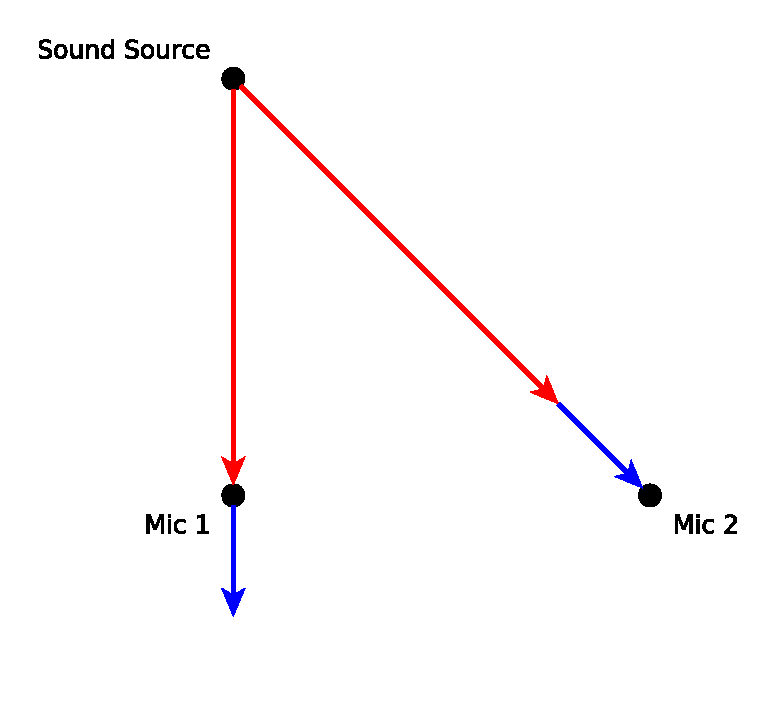
\includegraphics[width=0.66\textwidth]{diagrams/basics_ssl.pdf}
	\caption{Runtime variances for \gls{ssl}.
		A microphone array comprised of two microphones, Mic 1 and Mic 2, receive an audio signal from a sound source.
		When the signal of a particular event reaches Mic 1 (pictured in red), it is still on its way to Mic 2.
		When it reaches Mic 2 (pictured in blue), it has already passed Mic 1.}
	\label{pic:basics:ssl}
\end{figure}

\gls{ssl} requires an array of at least two microphones.
This will however yield two possible \gls{doa}, which may be enough, depending on the application.
To calculate an exact location in a two dimensional space, at least three microphones are needed, while a three dimensional space requires at least four.
An excess of microphones is often used in practice to increase accuracy of the \gls{doa}.

Due to practical limitations caused by slight inaccuracies in positioning of the microphones, an exact sound source can often only be determined in the immediate vicinity or even just inside of the microphone array.
Otherwise, only a general \gls{doa} can be calculated with respect to the microphone array.
Most approaches do not handle the special case of finding the exact position of a source inside the microphone array and thus only provide a \gls{doa}.

% todo: how to approaches to beamforming differ? maximum likelihood vs music

\section{Beamforming}
Beamforming \cite{beamforming2017} could colloquially be described as a sort of inverse of \gls{ssl}.
Its goal is to, in a way, "listen" to a particular direction and provide an audio signal given the recording of a number of microphones and a direction.
This new, artificial audio signal will greatly enhance audio events occurring in this particular direction.
Similarly to \gls{ssl}, a number of algorithms have been developed around a single principle, which will now be outlined.
\cite{1239145} provides an in-depth overview with regards to established beamforming techniques.

\begin{figure}[]
	\centering
	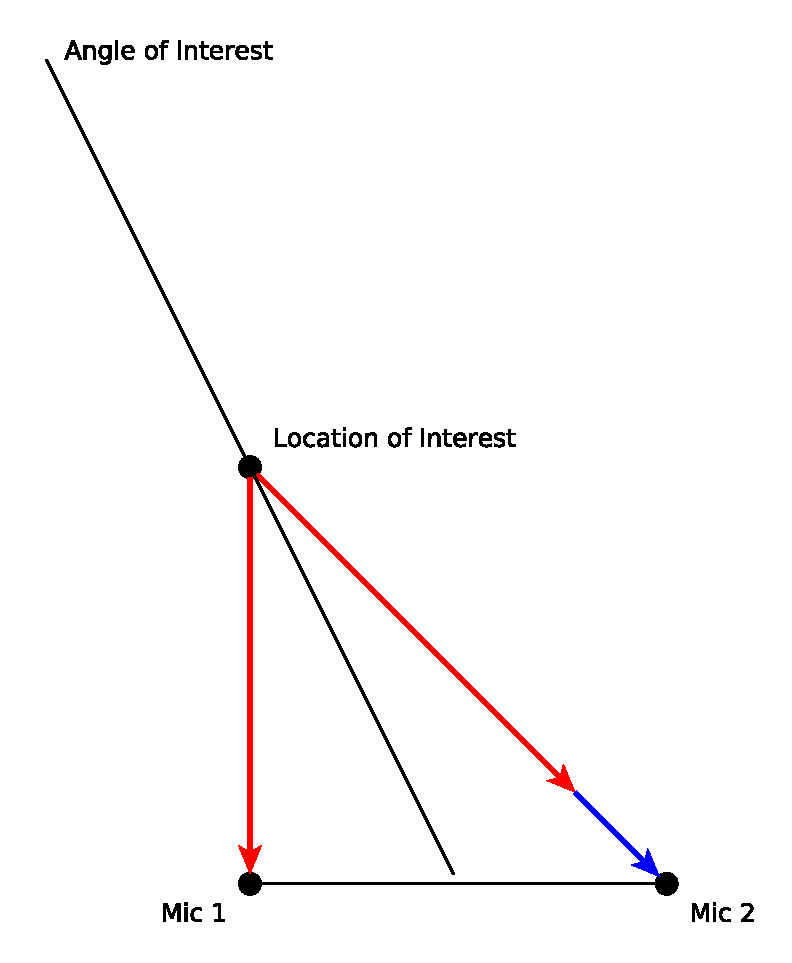
\includegraphics[width=0.49\textwidth]{diagrams/basics_beamforming.pdf}
	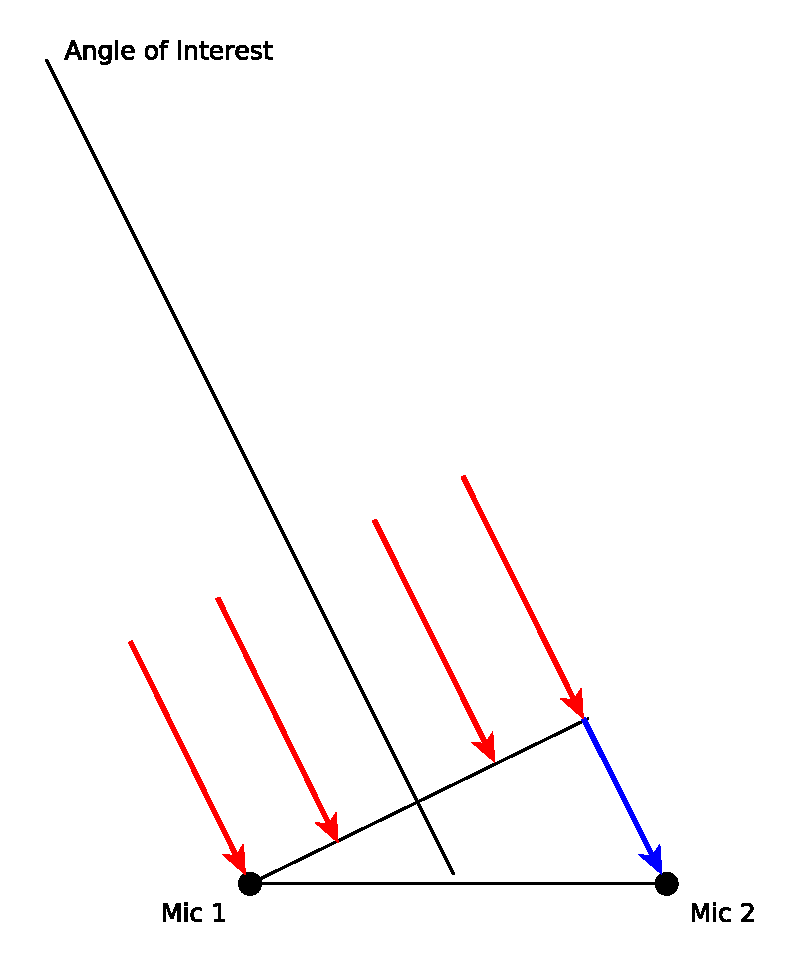
\includegraphics[width=0.49\textwidth]{diagrams/basics_beamforming_2.pdf}
	\caption{Beamforming with two microphones Mic 1 and Mic 2.
		On the left: By taking into account the additional time an audio event takes to reach Mic 2 (in blue), a new signal can be created, which greatly increases sound events originating from the location of interest.
		On the right: By the same principle, a location of interest infinitely far away can be targeted, which is then equivalent to improving sound events coming from a specific angle of interest.}
	\label{pic:basics:beamform}
\end{figure}

While in \gls{ssl} the source of the sound is not known and the time-of-arrival difference must be calculated from the signal, in beamforming the position of interest, or its angle relative to the microphone array is predetermined as seen in figure \ref{pic:basics:beamform}.
Due to this, one can compute the time-of-arrival difference expected by this position or angle, as indicated by the blue arrow.
By then combining the audio recorded from the microphones with respect to their positioning and expected time-of-arrival difference, one can create a new, virtual signal, which greatly improves the audio quality of events originating from this position or angle, while simultaneously greatly diminishing the events from distant positions or angles.
Beamforming can be used either together with \gls{ssl}, to improve sound quality from known sound sources, or independently from it, e.g. to focus on a person which had its position determined with the help of a camera.

\section{Robot Operating System}
\label{intro:ros}
\gls{ros} \cite{288} was developed explicitly for communication of programs in the context of robotics and offers a wide variety of standardized data types for transmission.
These include equivalents of widely used data types such as integer, float, char and string.
However, one is not limited to these data types, but can construct new types by combining already established ones.

Programs which make use of \gls{ros}, also called \gls{ros}-nodes, typically start by initializing \gls{ros} and thus announcing themselves to a dedicated \gls{ros}-master node, which orchestrates all communication within the \gls{ros} ecosystem and is always required.
They will then announce all their chosen ways of communication with other \gls{ros}-nodes and either start their work or await data or requests from other \gls{ros}-nodes.

\gls{ros} offers three distinct methods of transmitting these data types with increasing complexity:
the first is a simple one-way transmission of information\footnote{\url{http://archive.is/Tvsg7}}, from a so called \textit{Publisher}-node to a \textit{Subscriber}-node.
With it, data can be transmitted, also called published, to any number of \textit{Subscriber}-nodes.
Recipients are identified by the master-node by being subscribed to a specific communication channel, a so called topic, which must be the same as the one the \textit{Publisher}-node publishes to.

The second method is based on providing data on an on-demand basis and is know as a \gls{ros}\textit{-service}\footnote{\url{http://archive.is/ab2sd}}.
It features a \textit{service}-server, which advertises a specific \textit{service}.
Any \gls{ros}-node may then send this \textit{service}-server a request, which is, in essence, a \gls{ros} message.
The \textit{service}-server will then somehow react to this message and react with a single answer, another \gls{ros} message.
Similar to the simpler publish-subscribe method, \textit{services} are identified via a so called \textit{service}-topic.

The third method will be only discussed briefly, as it is not made use of in this work.
It is known as a \gls{ros} action\footnote{\url{http://archive.is/ujkJK}} and identifiable, similar to the already discussed methods, by an action-topic.
It is similar in nature to the \gls{ros} service, but features additional update messages send from the server to their respective client.

